\documentclass[./main.tex]{subfiles}

\begin{document}
\section{Experiment}\label{experiement}
Throughout the following section the results and configuration details of our trained model are described and explained. In the first section, Section \ref{subsec:conf_details}, the configuration details of the model, as well as the training of the model, are described. In the second section, Section \ref{subsec:results}, the results of training the Stacked hourglass is presented, as well as a short discussion of which version of the model which will be used going forward. In the last section, Section \ref{subsec:training_details}, we give an overview of the technical details behind training the network, which can be followed in case the reader has any technical problems in case of testing for reproducibility.

\subsection{Configuration Details}\label{subsec:conf_details}
Our model only consists of a single hourglass. The hourglass consists of $4$ down- and upsamples, with $1$ residual module between each down- and upsample. In each skip-connection a single residual module is used, and in the bottleneck $3$ residual modules are used. Newell \textit{et al.} \cite{Newell} and Olsen \cite{Camilla} experiment with different amount of hourglasses and with different amount of residual modules in each hourglass. They both come to the conclusion, that stacking multiple hourglasses or using hourglasses with multiple residual modules between each down- and upsample increases the performance of the model. However, as the main purpose of this thesis is not to create a model with state-of-the-art results, but instead to create a model that can be interpreted and explored, we have chosen to reduce the size of the model. For the same reasons, we will not be developing and testing various configurations of the architecture. Likewise, the purpose is neither to improve the model developed by Newell \textit{et. al} \cite{Newell}, hence why we will be making the same configuration choices as Newell \textit{et. al} \cite{Newell} and Olsen \cite{Camilla}, which are described in the following.
\\
\\
To prevent the model from overfitting we use batch normalization. Newell \textit{et al.} does not describe where to perform the batch normalization, so we follow Olsen \cite{Camilla} and perform the batch normalization before each convolutional layer in each residual module, after the first convolutional layer of the entire network and before the last convolutional layer of the entire network. For the choice of acitvation function we use the $ReLU$-function after each batch normalization. Each max pooling and nearest neighbor upsampling uses a kernel size of $2$, which halves and doubles the size of the input, respectively. The full network has been visualized in Figure \ref{fig:architecture}.
\\
\begin{figure}[p]
    \centering
    \begin{subfigure}{5 cm}
        \centering
        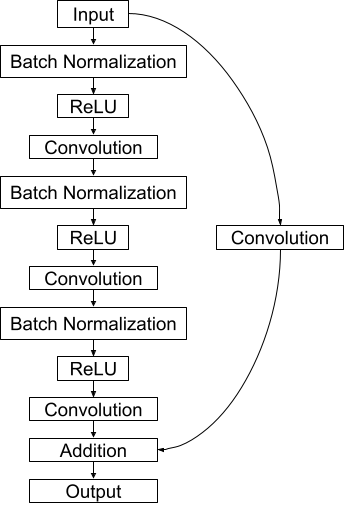
\includegraphics[width =  5 cm]{entities/residual_drawing.png}
        \caption{The Residual module}
    \end{subfigure}
    \begin{subfigure}{5 cm}
        \centering
        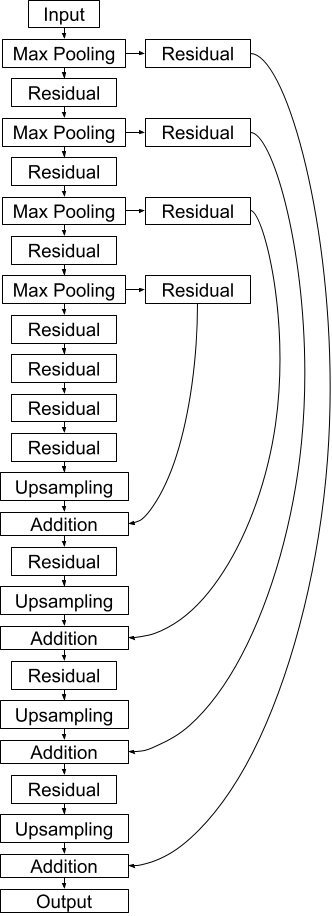
\includegraphics[width = 5 cm]{entities/hourglass_drawing.png}
        \caption{The Hourglass}
    \end{subfigure}
    \begin{subfigure}{5 cm}
        \centering
        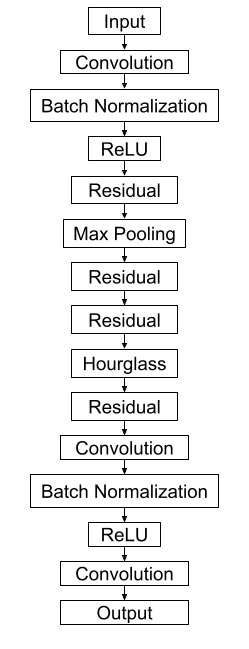
\includegraphics[width = 4 cm]{entities/SHG_drawing.png}
        \caption{The Full network}
    \end{subfigure}
    \caption{Overview of the used architecture}
    \label{fig:architecture}
\end{figure}
\\
For the initial values of the weights we initialize each weight by sampling from a \textit{Glorot normal distribution} (also known as a \textit{Xavier normal distribution}), described as
$$\mathcal{N} \left(0, \frac{2}{fan_{in} + fan_{out}} \right)$$
where $fan_{in}$ is the amount of input connections and $fan_{out}$ is the amount of output connections to the layer of the weight \cite{Xavier}. By doing so we make all layers have the same activation variance and gradient variance, essentially helping the model to converge \cite{DeepLearning}.
\\
\\
We make use of a mini-batch size of $16$ and no data augmentation, since the dataset is already rather large and captures a lot of the variances. To optimize the network we make use of $MSE$ as our loss function, \textit{RMSPROP} as our optimizer, as well as use a initial learning rate of $2.5e-4$. 
\\
\\
After each epoch we find the validation accuracy of the model by computing the \textit{PCK} between the predictions and the ground truth of the validation dataset, as described by Olsen \cite{Camilla} and the source code of the Stacked Hourglass Network \cite{SHG}, where it is called \textit{heatmap accuracy}.
\begin{algorithm}[t]
    \caption{PCK \cite{Camilla}\cite{SHG}}
    \label{Algorithm:PCK}
    \begin{algorithmic}[1]
        \Require Ground truth heatmaps $heatmaps_{gt}$ of keypoints
        \Require Predicted heatmaps $heatmaps_{pred}$ of keypoints
        \Require Threshold radius $r$
        \Require Normalization constant $c$
        \State Let $n = 0$ be the running total of correctly predicted keypoints
        \State Let $N \text{ be the amount of annotated heatmaps}$
        \ForAll{annotated ground truth heatmap, $heatmap_{gt}$, in $heatmaps_{gt}$}
            \State Let $(x_{gt}, y_{gt})$ be the $2D$ index of the maximum activation of $heatmap_{gt}$
            \State \begin{varwidth}[t]{\linewidth}
                Let $(x_{pred}, y_{pred})$ be the $2D$ index of the maximum activation of the predicted heatmap corresponding to $heatmap_{gt}$
            \end{varwidth}
            \State Let $dist$ be the Euclidean distance between $(x_{gt}, y_{gt})$ and $(x_{pred}, y_{pred})$.
            \State Normalize $dist$: $dist = \frac{dist}{c}$
            \If{$dist < r$}
                \State $n = n + 1$
            \EndIf
        \EndFor
        \State Let $ratio = \frac{n}{N}$ be the ratio of correctly annotated heatmaps
        \State \textbf{return} $ratio$
    \end{algorithmic}
\end{algorithm}
The pseudocode of PCK has been visualized in Algorithm \ref{Algorithm:PCK}. The algorithm works by iterating over each annotated ground truth heatmap and the corresponding predicted heatmap. It then finds the Euclidean distance between the maximum activation of a ground truth heatmap and the corresponding predicted heatmap. The distance is then normalized by a constant $c$ and compared to a threshold radius $r$. The ratio of normalized distances that are less than the threshold $r$ are then computed and returned, yielding the PCK accuracy between the ground truth heatmaps and the corresponding predicted heatmaps \cite{Camilla} \cite{SHG}. The aim is thus to maximize the PCK accuracy. To produce the final PCK accuracy of the model, the PCK accuracy is computed for each image in the validation dataset. The mean PCK accuracy is then used as the PCK accuracy of the model. For the two constants, $c$ and $r$, we let $c$ be one tenth of the heatmap resolution size $\left(\text{that is, }\frac{64}{10} = 6.4 \right)$ and $r$ be $0.5$.
\\
\\
While training the model the PCK accuracy of the model is computed after each epoch, keeping track of the best PCK accuracy. The first time the best PCK accuracy has not improved for $5$ continuous epochs, the learning rate is dropped by a factor of $5$ permanently, helping the training loss reach a minimum.

\subsection{Results}\label{subsec:results}
In Figure \ref{fig:results} the evolution of the training loss, validation loss and validation PCK accuracy has been visualized. The model were initially set to train for $100$ epochs, however, we decided to stop the training early, as the model clearly started to overfit after $32$ epochs, as seen by comparing the training and validation loss.
\\
\\
The reduction of the learning rate happened after $21$ epochs. By looking at the validation accuracy in Figure \ref{fig:results} we can see, that the accuracy rapidly increases shortly after the reduction of the learning rate, hinting at the effectiveness of dropping the learning rate. 
\\
\\
Comparing the training loss, validation loss and the validation accuracy from Table \ref{tab:results} we see, that the there is not an overlap between the models yielding the best training loss, validation loss and validation accuracy. As we in section \ref{sec:XAI} want to explore a model that performs decently well, we will be using the model with the highest validation accuracy as our model going forward. Thus, our model is the model from epoch $47$, which has a training loss of $4.19 \cdot 10^{-5}$, a validation loss of $5.43 \cdot 10^{-5}$ and a validation accuracy of $0.433$.
\begin{table}[b]
    \centering
    \begin{tabular}{|l|c|c|c|c|}
        \hline
        \textbf{Description} & \textbf{Epoch} & \textbf{Training loss} & \textbf{Validation loss} & \textbf{Validation accuracy} \\
        \hline
        Best training loss & $50$ & $4.11 \cdot 10^{-5}$ & $5.45 \cdot 10^{-5}$ & $0.43$ \\
        \hline
        Best validation loss & $32$ & $5.01 \cdot 10^{-5}$ & $5.15 \cdot 10^{-5}$ & $0.42$ \\
        \hline
        Best validation accuracy & $47$ & $4.19 \cdot 10^{-5}$ & $5.43 \cdot 10^{-5}$  & $0.433$ \\
        \hline
    \end{tabular}
    \caption{Comparison of the the epochs yielding the best training loss, validation loss and validation accuracy}
    \label{tab:results}
\end{table}

\begin{figure}[t]
    \centering
    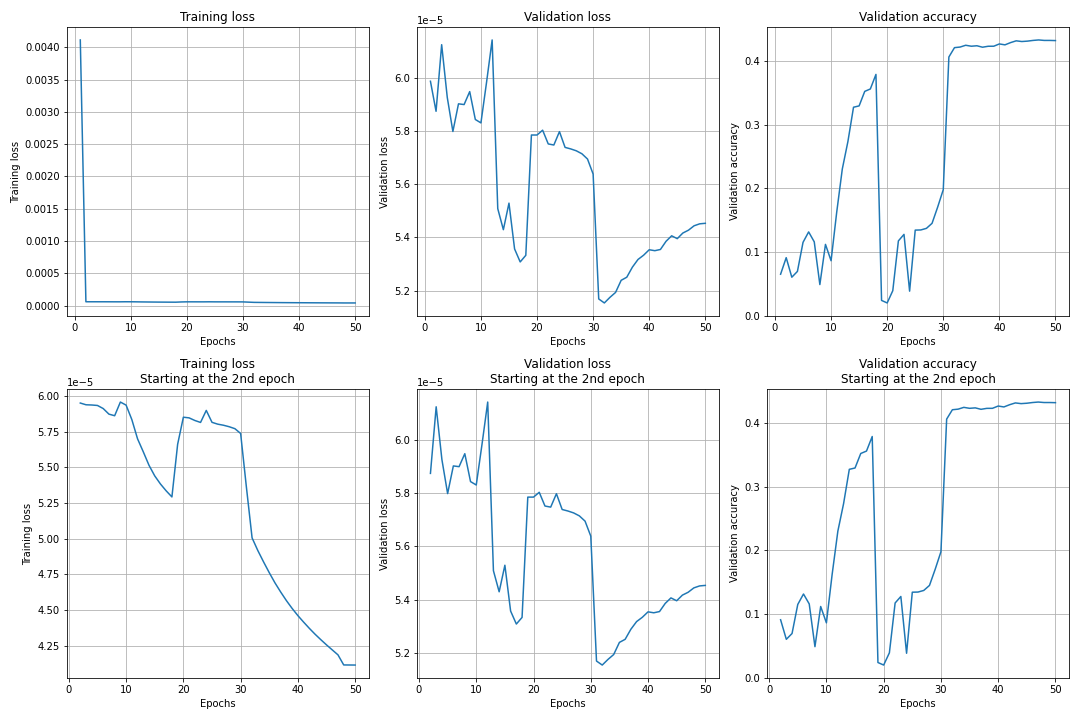
\includegraphics[width = \textwidth]{entities/results.png}
    \caption{Visualization of the evolution of the training loss, validation loss and validation PCK accuracy of the trained model. Top row shows all of the $50$ epochs. Bottom row shows epoch $2$ and forward to ease the reading of the training loss}
    \label{fig:results}
\end{figure}

\subsection{Training Details}\label{subsec:training_details}
The stacked hourglass was implemented in Python 3.8.2 using PyTorch version 1.7.1 and Cuda version 10.2 on a machine using Windows 10 version 20H2, build 19042. The network was trained on an 8 GB NVIDIA GeForce GTX 1070 GPU using a Samsung 840 EVO SSD for data storage. Training the network takes about $70$ minutes per epoch, totalling to about $58$ hours for $50$ epochs.

\end{document}